\chapter{Evaluation}
\label{ch:evaluation}

This chapter answers the research questions of \cref{ch:introduction} with measurements. Every
number below is inserted from the output of \code{experiments/run\_evaluation.py} and
\code{experiments/make\_figures.py}. \Cref{app:repro} explains how to regenerate them.

% ---------------------------------------------------------------------------
\section{Experimental setup}
\label{sec:eval:setup}

\paragraph{Model.} Unless stated otherwise, experiments use the \code{tiny} stub profile: four
blocks, hidden size 64, \TinyLayers{} weight tensors and \TinyParams{} INT8 parameters. The
small size keeps the full evaluation to about \WallTime{} seconds. Detection logic does not
depend on model size. Attestation cost does, and it is measured separately on larger profiles in
\cref{sec:eval:merkle}.

\paragraph{Activations.} Each of the \TinyLayers{} tensors is treated as a monitored layer with
an activation vector of dimension \ActDim{}, giving $m=\MChannels$ monitored channels. Clean
activations are drawn from $\mathcal{N}(10,5^2)$ clipped to INT8. Attack activations come from the
simulators of \cref{tab:simulators}.

\paragraph{Calibration and thresholds.} For each seed, the monitor is calibrated on \NCalib{}
fresh clean samples with full covariance ($d=\ActDim\le d_{\max}$). Thresholds are $\tau_z=4.0$,
$\tau_D=50$, $\theta_m=0.55$ and $\theta_H=0.30$.

\paragraph{Protocol.} There are ten scenarios: clean inputs, three bit-flip strategies, two
supply-chain strategies, two adversarial-input types, extraction probes and synergy attacks. For
each of \NSeeds{} seeds, a fresh detector is calibrated, and \NPerSeed{} inputs per scenario are
generated and classified, for \NPerScenario{} inputs per scenario in total. Every weight attack
starts from the clean weights, so each input carries exactly one attack.

\paragraph{Metrics.}
\begin{itemize}[leftmargin=*]
  \item \emph{Flag rate}: fraction of inputs given any label other than CLEAN. For attack
        scenarios this is the detection rate; for the clean scenario it is the false-positive rate.
  \item \emph{Label accuracy}: fraction given the label intended for the scenario.
  \item \emph{Monitor-only flag rate}: fraction for which the activation monitor alone reports
        an anomaly, ignoring attestation. This isolates what attestation adds.
  \item \emph{Exact localisation}: fraction of weight-modifying inputs for which the set of
        tensors reported as tampered equals the set actually changed, computed from a byte diff.
  \item \emph{Latency}: wall-clock time of the full \code{detect()} call, plus separately timed
        attestation and monitoring on the same inputs.
\end{itemize}
Means $\pm$ standard deviations are over the \NSeeds{} seeds.

\paragraph{Platform.} The machine was an x86-64 cloud container with \CPUCount{} virtual
CPUs, running Python \PyVer{} and NumPy \NpVer{}. All timings are single-threaded wall-clock
times on this machine, which has no NPU, and are reported only as relative costs.

% ---------------------------------------------------------------------------
\section{Overall results}

\begin{table}[t]
\centering
\caption{Detection results per scenario (\NPerScenario{} inputs each, mean $\pm$ s.d.\ over
\NSeeds{} seeds, in percentage points). ``Monitor only'' ignores attestation.}
\label{tab:results}
\small
\resizebox{\textwidth}{!}{% AUTO-GENERATED
\begin{tabular}{lrrrrr}
\toprule
\textbf{Scenario} & \textbf{Monitor only} & \textbf{Flagged} & \textbf{Correct label} & \textbf{Mean (ms)} & \textbf{p99 (ms)} \\
\midrule
Clean (no attack) & 7.2\% & 7.2\% $\pm$ 1.5 & 92.8\% $\pm$ 1.5 & 1.57 & 3.36 \\
BFA, random bit & 7.9\% & 100.0\% $\pm$ 0.0 & 100.0\% $\pm$ 0.0 & 1.61 & 3.11 \\
BFA, sign bit & 7.7\% & 100.0\% $\pm$ 0.0 & 100.0\% $\pm$ 0.0 & 1.52 & 2.53 \\
BFA, progressive & 7.7\% & 100.0\% $\pm$ 0.0 & 100.0\% $\pm$ 0.0 & 1.59 & 2.60 \\
Supply chain, LSB stego & 6.9\% & 100.0\% $\pm$ 0.0 & 0.0\% $\pm$ 0.0 & 1.60 & 2.99 \\
Supply chain, distributed & 7.3\% & 100.0\% $\pm$ 0.0 & 100.0\% $\pm$ 0.0 & 1.63 & 2.84 \\
Adversarial, text injection & 100.0\% & 100.0\% $\pm$ 0.0 & 100.0\% $\pm$ 0.0 & 1.60 & 2.68 \\
Adversarial, safety bypass & 100.0\% & 100.0\% $\pm$ 0.0 & 0.0\% $\pm$ 0.0 & 1.61 & 2.55 \\
Training-data exfil.\ probe & 100.0\% & 100.0\% $\pm$ 0.0 & 100.0\% $\pm$ 0.0 & 1.68 & 3.79 \\
Synergy (BFA + adversarial) & 4.7\% & 100.0\% $\pm$ 0.0 & 100.0\% $\pm$ 0.0 & 1.54 & 3.29 \\
\bottomrule
\end{tabular}
}
\end{table}

\begin{figure}[t]
\centering
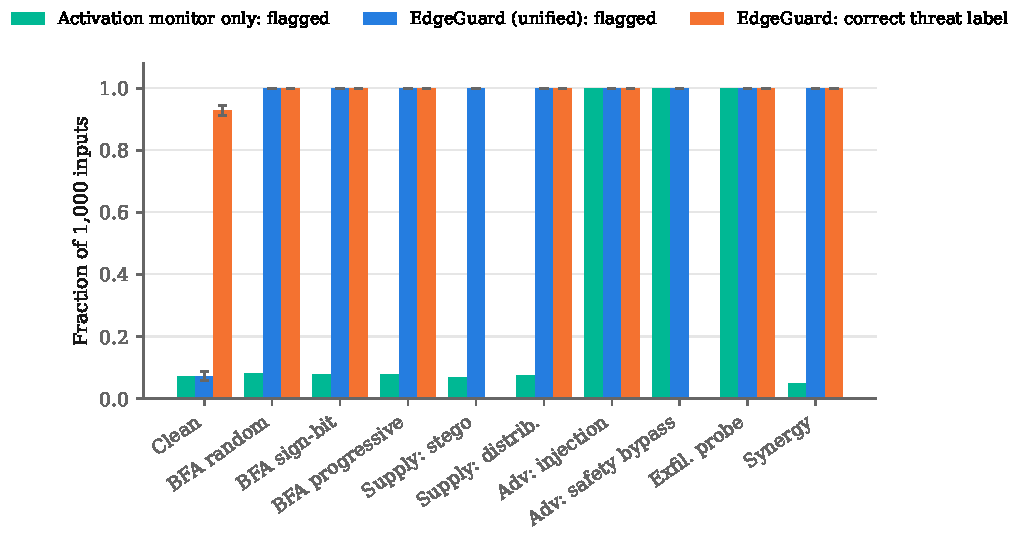
\includegraphics[width=\textwidth]{detection_by_scenario.pdf}
\caption{Per-scenario outcomes. Green: activation monitor alone. Blue: full \textsc{EdgeGuard}
pipeline. Orange: fraction receiving the intended label. Error bars: s.d.\ over seeds.}
\label{fig:detection}
\end{figure}

\Cref{tab:results} and \cref{fig:detection} summarise the outcomes. Three patterns stand out
and are examined in turn below. All weight-modifying scenarios are flagged on every input, while
the monitor alone flags them at roughly its clean false-positive rate. All activation-level
scenarios are flagged on every input by both. And label accuracy is perfect in six of the nine
attack scenarios but zero in two.

% ---------------------------------------------------------------------------
\section{RQ1: weight integrity and localisation}
\label{sec:eval:rq1}

Every input in the six weight-modifying scenarios was flagged: \FlagBfaRandom{} for random bit
flips, \FlagBfaSignBit{} for sign-bit flips, \FlagBfaProgressive{} for progressive flips,
\FlagSupplySteg{} for steganographic LSB poisoning, \FlagSupplyDistributed{} for distributed
poisoning and \FlagSynergy{} for synergy attacks. The tensors reported as tampered matched the
byte-level ground truth exactly in every case. This includes the distributed scenario, where up
to all \TinyLayers{} tensors change, and the steganographic scenario, where only up to 16
least-significant bits of one tensor change.

These results confirm \cref{prop:integrity,prop:localise} empirically, but they should not be
over-read. They are a correctness check of the implementation, not a discovery. Any change to a
byte changes a SHA-256 digest. The value of the experiment lies in confirming that the
implementation hashes what it should, in the right order, with the shape included, and that
localisation is exact for every attack pattern the simulators produce.

The monitor-only column shows the other side. Weight attacks leave the simulated activations
untouched, because the simulators do not propagate weight changes into activations, so the
monitor flags these inputs at rates between \MonSupplySteg{} and \MonBfaRandom{},
indistinguishable from its clean rate of \MonClean{}. In a real model, a damaging bit flip would usually perturb activations
downstream, but a carefully chosen one might not. Attestation does not depend on that question.

% ---------------------------------------------------------------------------
\section{RQ2: activation anomalies and the false-positive rate}
\label{sec:eval:fpr}

\subsection{Separation of attack activations}

The monitor flagged \MonAdvTextInjection{} of text-injection inputs, \MonAdvSafetyBypass{} of
safety-bypass inputs and \MonExfilProbe{} of extraction probes. The ROC curves of the
input-level maximum $|z|$ statistic (\cref{fig:roc}) have an AUC of 1.00 for all three. The
attack and clean score distributions do not overlap at all.

\begin{figure}[t]
\centering
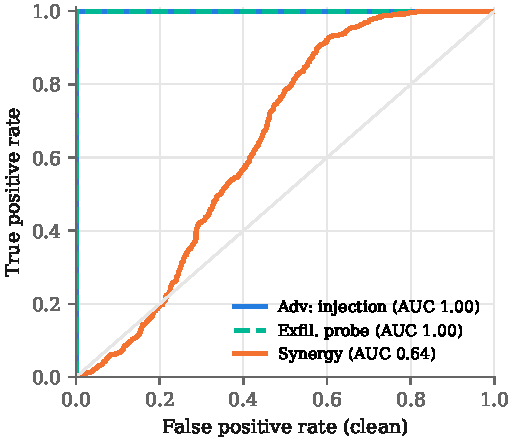
\includegraphics[width=0.62\textwidth]{roc_activation_monitor.pdf}
\caption{ROC curves of the maximum $|z|$ statistic, attack inputs against clean inputs
(\NPerScenario{} each). The safety-bypass curve coincides with the text-injection curve and is
omitted.}
\label{fig:roc}
\end{figure}

\begin{figure}[t]
\centering
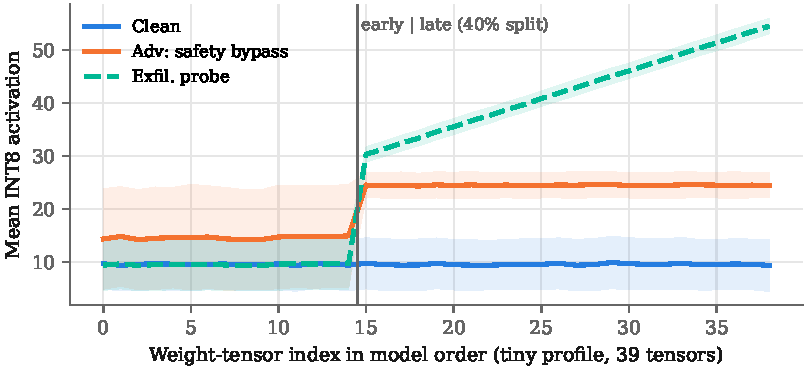
\includegraphics[width=\textwidth]{activation_profiles.pdf}
\caption{Mean INT8 activation per tensor index (50 samples; bands $\pm1$ s.d.) for clean
inputs, safety-bypass inputs and extraction probes, as produced by the simulators.}
\label{fig:profiles}
\end{figure}

Perfect separation is expected given how the attacks are simulated, and \cref{fig:profiles}
shows why. Text injection and safety bypass inflate the early-layer standard deviation from 5 to
12.5 and 10 respectively, so each early channel has a probability of several per cent of exceeding
$|z|=4$, and with 15 early layers of 32 channels at least one almost surely does. The extraction
probe moves late-layer means to between 15 and 55, which is up to nine clean standard deviations
from the clean mean of 10. A maximum-$z$ detector cannot miss either pattern. The experiment shows that the scoring and
decision path works. It does not show that real adversarial inputs or real extraction probes
produce shifts of this size. Real adversarial perturbations are typically optimised to be
small, and an adaptive attacker would aim to stay inside the calibration region
(\cref{sec:disc:adaptive}).

\subsection{The false-positive rate is a multiple-comparisons effect}

On clean inputs the pipeline raised an alarm on \FlagClean{} of inputs (\cref{tab:results}).
Of the clean inputs, \CleanAdvFrac{} were labelled ADVERSARIAL\_INPUT and \CleanTFFrac{}
TRANSIENT\_FAULT. A 7\% false-positive rate would be unacceptable in deployment, so its cause
matters.

Each monitored channel is compared against $\tau_z=4$. Under a Gaussian model, a single channel
exceeds this two-sided threshold with probability $\PSingleZFour$, but an input is flagged if any
of its $m=\MChannels$ channels does. \Cref{eq:fwer} then predicts a false-positive rate of
\PredFPRZFour{}. The measured rate was \EmpFPRZFour{}. \Cref{fig:fpr} compares the predicted and
measured rates across all thresholds from 2.5 to 6. The two curves nearly coincide, which shows
that the false-positive rate is almost entirely explained by the number of comparisons, with
channel independence and approximate Gaussianity holding well in this simulation.

\begin{figure}[t]
\centering
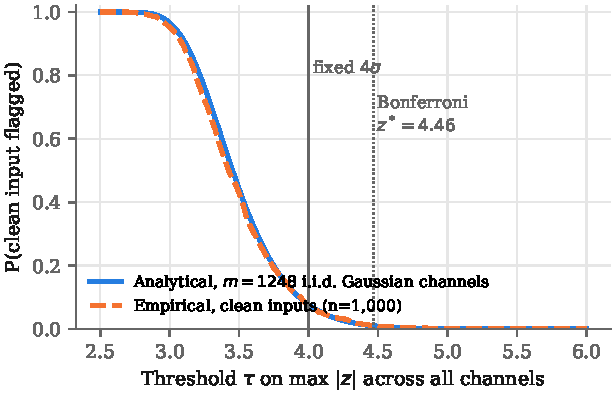
\includegraphics[width=0.75\textwidth]{fpr_multiple_comparisons.pdf}
\caption{Probability that a clean input is flagged by the $z$ test, as a function of the
threshold. Analytical: \cref{eq:fwer} with $m=\MChannels$. Empirical: \NPerScenario{} clean
inputs. Vertical lines: the default $\tau_z=4$ and the Bonferroni threshold for $\alpha=1\%$.}
\label{fig:fpr}
\end{figure}

\begin{figure}[t]
\centering
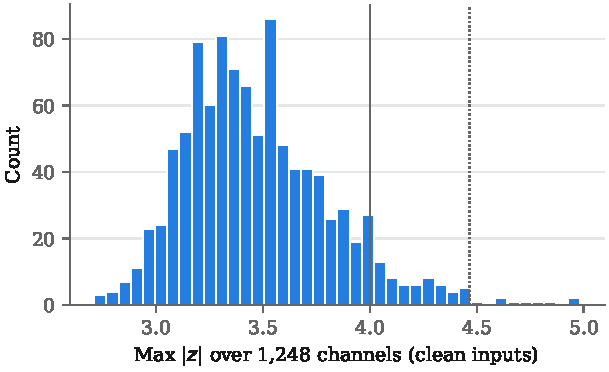
\includegraphics[width=0.7\textwidth]{clean_maxz_histogram.pdf}
\caption{Distribution of the input-level maximum $|z|$ over \MChannels{} channels for clean
inputs. Solid line: $\tau_z=4$; dotted line: $z^*=\ZBonf$.}
\label{fig:maxz}
\end{figure}

\Cref{fig:maxz} shows the same effect directly. For clean inputs the maximum $|z|$ over all
channels averaged \CleanMaxZMean{}, close to the \ExpMaxGauss{} expected for the largest of
\MChannels{} standard-normal magnitudes, and its 99th percentile was \CleanMaxZPNinetyNine{}. A
threshold of 4 therefore sits inside the bulk of the clean distribution of the statistic that
the monitor actually tests.

\subsection{A corrected threshold}

The Bonferroni threshold \cref{eq:bonf} for a target input-level false-positive rate of 1\% is
$z^*=\ZBonf$. Applying it to the recorded scores gave:

\begin{itemize}[leftmargin=*]
  \item a clean false-positive rate of \EmpFPRBonf{}, against a target of 1\%;
  \item 100\% detection of text-injection, safety-bypass and extraction-probe inputs, unchanged;
  \item \SynergyTPRBonf{} monitor-only detection of synergy inputs.
\end{itemize}

Because the activation-level attacks are so strongly separated, the threshold can be raised
without loss in this simulation. The general lesson does not depend on the simulation: a
detector that takes a maximum over many channels must set its threshold for the maximum, not for
a single channel. Doing so requires only the channel count. Monitoring a real language model,
with thousands of channels per layer and dozens of layers, would push $m$ into the hundreds of
thousands, and a per-channel $4\sigma$ rule would flag almost every input. The corrected threshold
grows only slowly with $m$, roughly as $\sqrt{2\ln m}$.

% ---------------------------------------------------------------------------
\section{RQ3: complementarity and the synergy attack}
\label{sec:eval:synergy}

The synergy scenario combines a targeted sign-bit flip with a safety-bypass input whose
activations are blended toward clean ones. The monitor alone flagged \MonSynergy{} of synergy
inputs, below its own clean false-positive rate of \MonClean{}. The blend pulls early layers back
to approximately the clean distribution, and it leaves late layers at a mean near 19 with a
standard deviation near 2. That is about two clean standard deviations above the mean but with
\emph{less} spread than clean data, so extreme channels are rarer than on clean inputs. The ROC AUC of the $|z|$ statistic against clean inputs was \AUCSynergy{}
(\cref{fig:roc}): the blended activations sit slightly above the clean distribution but overlap
it heavily. At the Bonferroni threshold, monitor-only detection fell to \SynergyTPRBonf{}. The
full pipeline flagged \FlagSynergy{} of synergy inputs and labelled all of them WEIGHT\_TAMPER,
because attestation sees the flipped bit regardless of the activations.

This is the complementarity predicted in \cref{sec:design:complement}. It is a demonstration
rather than an empirical finding about real attackers: the simulator sets the degree of
suppression directly. The result shows that the pipeline is wired so that weight evidence
overrides weak activation evidence, and that an activation monitor alone would have missed these
inputs.

% ---------------------------------------------------------------------------
\section{RQ4: threat labels}
\label{sec:eval:labels}

\begin{figure}[t]
\centering
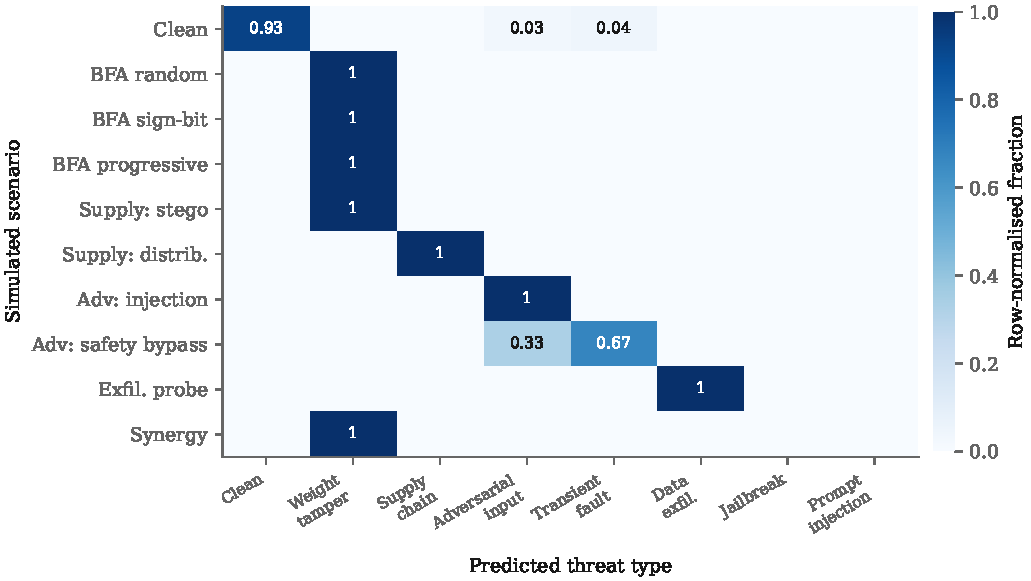
\includegraphics[width=\textwidth]{confusion_matrix.pdf}
\caption{Row-normalised confusion matrix of scenario (rows) against assigned label (columns),
\NPerScenario{} inputs per row. Raw counts are in \cref{app:results}.}
\label{fig:confusion}
\end{figure}

\Cref{fig:confusion} shows the full label distribution. Six of the nine attack scenarios received
their intended label on every input: the three bit-flip strategies (WEIGHT\_TAMPER),
distributed poisoning (SUPPLY\_CHAIN\_BACKDOOR), text injection (ADVERSARIAL\_INPUT) and
extraction probes (TRAINING\_DATA\_EXFILTRATION). Synergy inputs were labelled WEIGHT\_TAMPER,
which is the intended label because the weight evidence takes priority. Two scenarios were
labelled wrongly every time, for different reasons.

\paragraph{Steganographic poisoning was labelled WEIGHT\_TAMPER.} The supply-chain label requires
more than 30\% of tensors to be modified, and the steganographic simulator modifies one. From the
weights alone, a single modified tensor looks exactly like a runtime bit flip. This is a
limitation of the rule rather than a defect in its implementation: weights carry no record of
when or how they were changed. Distinguishing supply-chain tampering from runtime tampering
would require temporal evidence. For example, verifying at load time and again periodically
would separate weights that were wrong from the start from weights that changed in memory. With
that information, the label could be assigned correctly even for one-tensor modifications.

\paragraph{Safety-bypass inputs were never labelled JAILBREAK.} \SafetyAdvFrac{} were labelled
ADVERSARIAL\_INPUT and \SafetyTFFrac{} TRANSIENT\_FAULT. Two separate issues combine here.
\begin{enumerate}[leftmargin=*]
  \item The JAILBREAK and PROMPT\_INJECTION labels require the late-layer entropy to fall below
        0.30. The safety-bypass simulator shifts late activations upward and narrows them, but
        the entropy of \cref{eq:entropy} is invariant to shifts and to rescaling, and the
        simulated activations never come close to the threshold. The entropy branch was
        therefore never taken in any scenario. Either the score or the simulator, or both, would
        need redesign before this branch could be evaluated.
  \item Falling through to the base classifier, the early share decides the label. The 15 early
        layers, with standard deviation 10, are essentially always anomalous. The 24 late layers,
        at mean 25 and standard deviation 2.5, sit about three clean standard deviations above
        the mean, and each crosses $\tau_z=4$ only when one of its channels lands in the upper
        tail. With $k$ anomalous late layers, the early share is $15/(15+k)$, and the label is
        ADVERSARIAL\_INPUT only if $k\le15$. The split of roughly one third to two thirds
        reflects how often more than 15 late layers cross the threshold. It is the bias
        anticipated in \cref{sec:design:classifier}: the more thoroughly an input disturbs the
        network, the more likely it is to be called a fault.
\end{enumerate}
Comparing the anomaly \emph{rate} among early layers with that among late layers, rather than the
share of anomalies that are early, would label inputs that are anomalous everywhere as
adversarial rather than as faults. This change, together with a redesigned entropy score, is part
of the plan in \cref{ch:conclusion}.

\paragraph{Clean false positives were split} between ADVERSARIAL\_INPUT (\CleanAdvFrac{}) and
TRANSIENT\_FAULT (\CleanTFFrac{}), in roughly the ratio of early to late layers. This is
consistent with false alarms caused by single extreme channels located uniformly at random.

% ---------------------------------------------------------------------------
\section{RQ5: cost}
\label{sec:eval:cost}

\subsection{Per-inference latency on the tiny profile}

\begin{figure}[t]
\centering
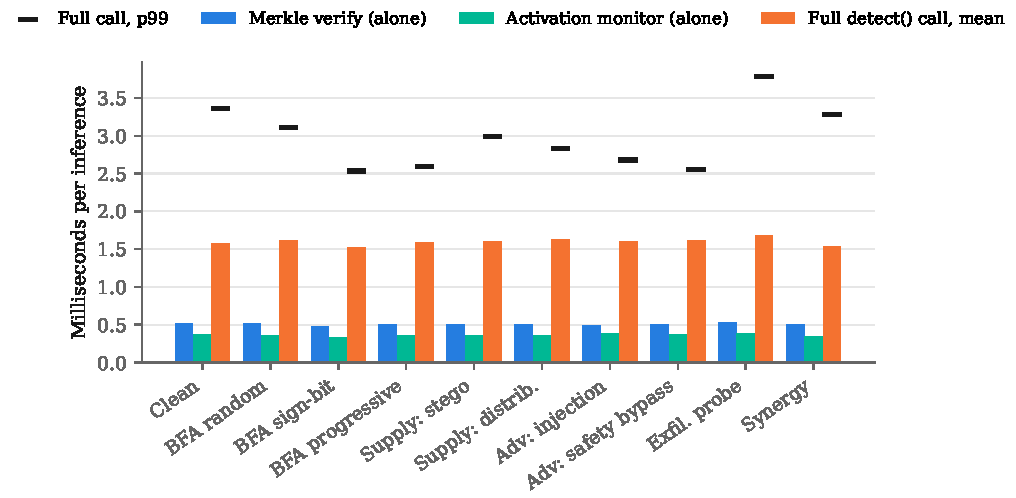
\includegraphics[width=\textwidth]{latency_breakdown.pdf}
\caption{Per-inference latency on the tiny profile: attestation alone, monitoring alone and the
full \code{detect()} call (mean, with p99 marked).}
\label{fig:latency}
\end{figure}

\Cref{fig:latency} breaks down the latency. The full \code{detect()} call took between
\LatMin{} and \LatMax{}\,ms on average across scenarios, with p99 values of at most \LatPMax{}\,ms. Attestation
alone took about \AttClean{}\,ms, which covers re-hashing all \TinyLayers{} tensors (about
0.36\,MiB) and one ECDSA verification of the reference root.
Monitoring alone took about \MonMsClean{}\,ms for \TinyLayers{} layers with $32\times32$
covariance products. The remaining time of the full call, a little under half, is spent in the
LLM scores, the classifier and building explanation strings. That share is pure overhead of the
prototype and could be reduced, for example by building explanations only when an alarm is
raised.

\subsection{Attestation cost at language-model scale}
\label{sec:eval:merkle}

\begin{table}[t]
\centering
\caption{Attestation cost on stub weight sets of increasing size (mean of three verifications;
single-threaded, 2-vCPU x86 container). The last column confirms that a single-bit change in the
last block's \code{down\_proj} was detected and localised to that tensor.}
\label{tab:merkle}
\small
\resizebox{\textwidth}{!}{% AUTO-GENERATED
\begin{tabular}{lrrrrrc}
\toprule
\textbf{Stub profile} & \textbf{Tensors} & \textbf{Params} & \textbf{MiB} & \textbf{Build (ms)} & \textbf{Verify (ms)} & \textbf{1-bit tamper localised} \\
\midrule
TinyLLM-INT8 & 39 & 366{,}144 & 0.3 & 0.7 & 0.4 & yes \\
Qwen2.5-0.5B-INT8 & 219 & 627{,}387{,}264 & 598.3 & 661.8 & 575.6 & yes \\
Llama-3.2-1B-INT8 & 147 & 1{,}469{,}122{,}560 & 1401.1 & 1605.7 & 1578.3 & yes \\
\bottomrule
\end{tabular}
}
\end{table}

\begin{figure}[t]
\centering
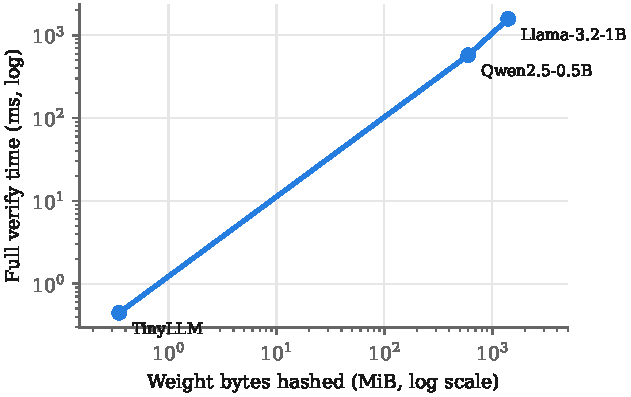
\includegraphics[width=0.65\textwidth]{merkle_scaling.pdf}
\caption{Full attestation time against the number of weight bytes hashed (log--log). Time is
linear in bytes, at roughly \MerkThrMin{}--\MerkThrMax{}\,MiB/s on this machine.}
\label{fig:merkle_scaling}
\end{figure}

\Cref{tab:merkle} and \cref{fig:merkle_scaling} report full build and verify times for three stub
profiles. Verification time is linear in the number of bytes, at \MerkThrMin{}--\MerkThrMax{}\,MiB/s
for the larger sets, which is SHA-256 throughput on one core. Verifying the Qwen2.5-0.5B stub
(\MerkSizeQwenPPB{}\,MiB) took \MerkVerQwenPPB{}\,ms; verifying the Llama-3.2-1B stub
(\MerkSizeLlamaPB{}\,MiB) took \MerkVerLlamaPB{}\,ms. A single-bit modification was detected and
localised correctly in all three.

These numbers settle RQ5 in one direction. Full re-attestation on every inference is practical
for small models but not for language models. An on-device LLM generating tokens at tens of
milliseconds per token cannot afford a 1.6-second hash pass per token. Even with hardware SHA
extensions several times faster than this container, full attestation must be amortised.
\Cref{sec:disc:amortise} discusses how the Merkle structure supports this.

% ---------------------------------------------------------------------------
\section{Fidelity of simulated weight extraction}
\label{sec:eval:extraction}

\begin{table}[t]
\centering
\caption{Cosine similarity between the dequantized extracted weights and the originals, averaged
over the tiny profile's tensors and \NSeeds{} seeds.}
\label{tab:extraction}
\small
% AUTO-GENERATED
\begin{tabular}{lrr}
\toprule
\textbf{Channel model} & \textbf{Mean cosine fidelity} & \textbf{Std.\ over seeds} \\
\midrule
Memory dump (no noise) & 1.00000 & 0.0e+00 \\
Cold boot (0.2\% single-bit decay) & 0.98772 & 7.2e-03 \\
EM side channel (2.5\% $\pm 1$ LSB) & 0.99999 & 3.0e-07 \\
\bottomrule
\end{tabular}

\end{table}

\Cref{tab:extraction} reports how closely each simulated extraction channel reproduces the
weights. A memory dump is exact. The EM channel model, which perturbs 2.5\% of weights by one
LSB, still yields a cosine similarity of \FidEmSideChannel{}, because a one-LSB error on a value
of typical magnitude around 25 is tiny. The cold-boot model, which flips one random bit in 0.2\%
of bytes, yields \FidColdBoot{}. It perturbs fewer weights, but its flips include high-order
and sign bits, each worth up to 128 units. An earlier version of this experiment, before the fix
in \cref{sec:impl:bugs}, saturated sign-bit decays instead of wrapping them, which distorts
exactly this comparison.

The practical reading is that an attacker who can read DRAM even imperfectly obtains an
essentially faithful copy of an INT8 model. Error rates would have to be far higher than those
modelled here before the copy became useless. This supports the case for confidentiality
mechanisms such as Amulet \cite{mao2025amulet}, which \textsc{EdgeGuard} does not provide.

% ---------------------------------------------------------------------------
\section{Summary}
\label{sec:eval:summary}

\begin{table}[t]
\centering
\caption{Answers to the research questions, with the strength of the evidence.}
\label{tab:rq_summary}
\small
\begin{tabularx}{\textwidth}{@{}p{1.2cm}Xp{3.2cm}@{}}
\toprule
\textbf{RQ} & \textbf{Finding} & \textbf{Evidence} \\
\midrule
RQ1 & All weight modifications detected; modified tensors localised exactly. & Strong; independent of simulation. \\
RQ2 & Simulated attacks separated perfectly. A fixed $4\sigma$ rule gives a \EmpFPRZFour{} FPR, explained by multiple comparisons; Bonferroni gives \EmpFPRBonf{}. & FPR analysis strong; separation limited by simulation. \\
RQ3 & Synergy inputs evade the monitor (\MonSynergy{}) but not the combined pipeline (\FlagSynergy{}). & Demonstration; suppression set by simulator. \\
RQ4 & Intended label in 6 of 9 attack scenarios. Steganographic poisoning indistinguishable from BFA; jailbreak branch unreachable; early/late rule biased. & Strong for the identified failures. \\
RQ5 & Detection call 1.5--1.7\,ms on tiny model. Attestation at \MerkThrMin{}--\MerkThrMax{}\,MiB/s, 1.6\,s for 1.4\,GiB: per-inference attestation infeasible for LLMs. & Strong on this machine; NPU untested. \\
\bottomrule
\end{tabularx}
\end{table}

\Cref{tab:rq_summary} collects the answers. The strongest results are those that do not depend
on how activations were simulated: exact detection and localisation of weight changes, the
explanation of the false-positive rate and its correction, and the cost of attestation at scale.
The activation-level detection rates and the synergy result show that the pipeline works as
designed, but they need real-model data before they can support claims about real attacks.
